\section{Research model} \label{research_model}

When decomposing the statements made in section \ref{sec:research_relevance}
\nameref{sec:research_relevance} and the \nameref{sec:research_questions} the cause and
effect relationship between the independent-, and dependent variable can be determined. It
is clear that the independent variable 'Clean Architecture' has an effect on the outcome
of the design article that has been described in \ref{chap:artifact_design}
\nameref{chap:artifact_design}. 

Since there is plentiful scientific proof, the Normalized Systems theorems are used as the
baseline to measure the results. In the overall conceptual research framework, Normalized
Systems Theorems are considered to be the Moderator variable. In the context of this
research, Clean Architecture does not have a causal effect on Normalized Systems.

Since this research intends to demonstrate the level of convergence of Clean Architecture
with Normalized Systems, modularity, stability and evolvability are positioned as the
Mediator variable in this conceptual framework.

Figure \ref{fig:conceptual_framework} \nameref{fig:conceptual_framework} depicts a
graphical representation of the overall conceptual framework described above.

\begin{figure}[H]
    \centering
    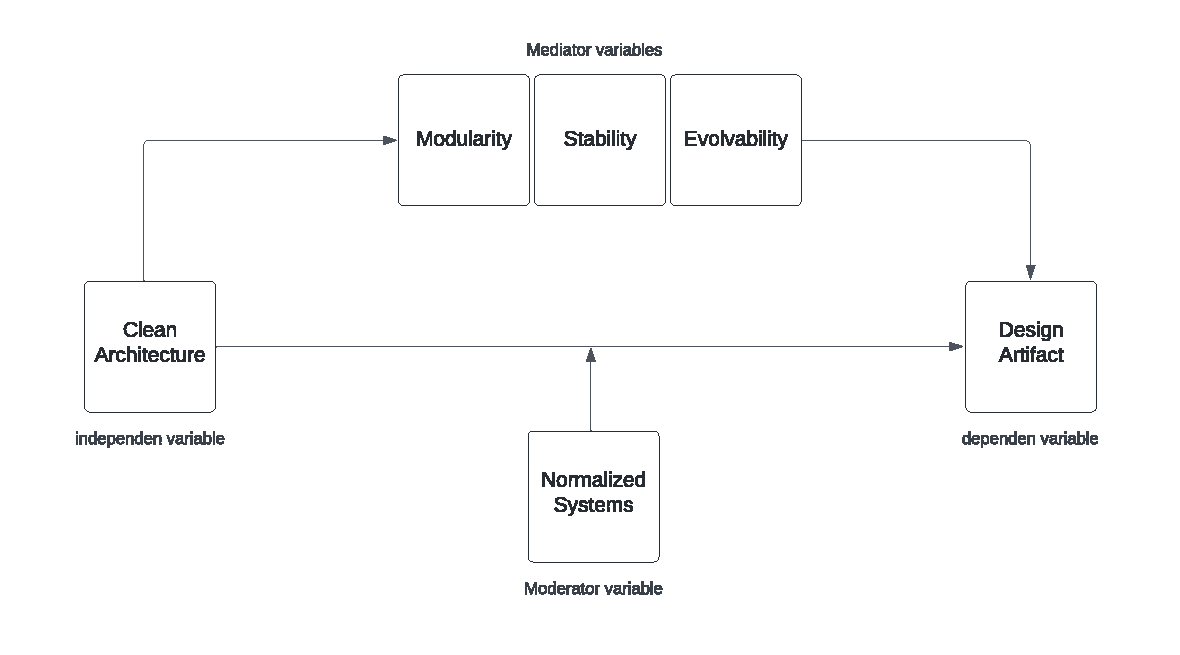
\includegraphics[width=1\textwidth]{Figures/conceptual_framework}
    \caption[Overall conceptual framework]{Overall conceptual framework}
    \label{fig:conceptual_framework}
\end{figure}
